\documentclass[11pt,letterpaper]{article}
\usepackage[utf8]{inputenc}
\usepackage[T1]{fontenc}
\usepackage{amsmath,amssymb,amsfonts}
\usepackage{graphicx}
\usepackage{booktabs}
\usepackage{array}
\usepackage{longtable}
\usepackage{geometry}
\usepackage{xcolor}
\usepackage{tikz}
\usetikzlibrary{shapes.geometric, arrows.meta, positioning, calc, decorations.pathreplacing}
\usepackage{tcolorbox}
\usepackage{enumitem}
\usepackage{fancyhdr}
\usepackage{titlesec}
\usepackage{hyperref}
\usepackage{multirow}
\usepackage{colortbl}
\usepackage{float}

\geometry{margin=1in}

% Color definitions
\definecolor{asumaroon}{RGB}{140,29,64}
\definecolor{asugold}{RGB}{255,198,39}
\definecolor{darkblue}{RGB}{31,78,121}
\definecolor{lightblue}{RGB}{213,232,240}
\definecolor{lightgray}{RGB}{245,245,245}
\definecolor{vmgreen}{RGB}{119,185,0}
\definecolor{vmpurple}{RGB}{102,45,145}

% Header/Footer
\pagestyle{fancy}
\fancyhf{}
\fancyhead[L]{\small\textcolor{asumaroon}{GTFS2GMNS Transit System Modeling}}
\fancyhead[R]{\small\textcolor{asumaroon}{Transportation+AI Lab}}
\fancyfoot[C]{\thepage}
\renewcommand{\headrulewidth}{0.5pt}

% Section formatting
\titleformat{\section}{\Large\bfseries\color{darkblue}}{\thesection}{1em}{}
\titleformat{\subsection}{\large\bfseries\color{asumaroon}}{\thesubsection}{1em}{}
\titleformat{\subsubsection}{\normalsize\bfseries\color{darkblue}}{\thesubsubsection}{1em}{}

% Custom boxes
\tcbuselibrary{skins,breakable}
\newtcolorbox{deliverablebox}[1]{
    colback=lightblue, 
    colframe=darkblue, 
    fonttitle=\bfseries,
    title=#1,
    breakable
}
\newtcolorbox{metricbox}[1]{
    colback=asugold!20, 
    colframe=asugold!80!black, 
    fonttitle=\bfseries,
    title=#1,
    breakable
}
\newtcolorbox{conceptbox}[1]{
    colback=lightgray, 
    colframe=asumaroon, 
    fonttitle=\bfseries,
    title=#1,
    breakable
}
\newtcolorbox{readingbox}[1]{
    colback=vmgreen!10, 
    colframe=vmgreen!80!black, 
    fonttitle=\bfseries,
    title=#1,
    breakable
}
\newtcolorbox{warningbox}[1]{
    colback=red!5, 
    colframe=red!70!black, 
    fonttitle=\bfseries,
    title=#1,
    breakable
}

\begin{document}

% Title Page
\begin{titlepage}
\centering
\vspace*{1.5cm}

{\Huge\bfseries\color{asumaroon} GTFS2GMNS\\[0.3cm] Transit System Modeling}\\[0.5cm]
{\Large\color{darkblue} From Data Conversion to Decision Variables}\\[1.5cm]

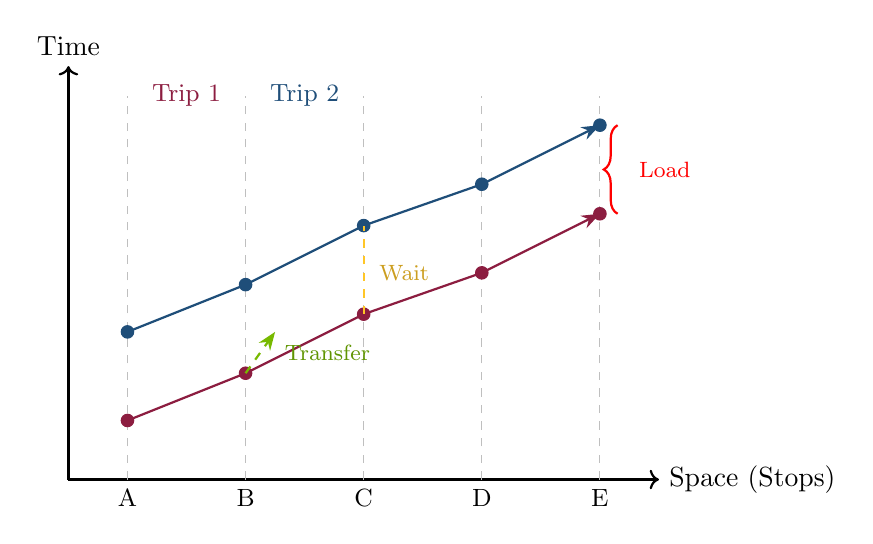
\begin{tikzpicture}[scale=0.75]
% Time-space diagram illustration
\draw[thick, ->] (0,0) -- (10,0) node[right] {Space (Stops)};
\draw[thick, ->] (0,0) -- (0,7) node[above] {Time};

% Stops
\foreach \x/\label in {1/A, 3/B, 5/C, 7/D, 9/E} {
    \draw[dashed, gray!50] (\x,0) -- (\x,6.5);
    \node[below] at (\x,0) {\small\label};
}

% Trip 1 (Bus line)
\draw[thick, asumaroon, -Stealth] (1,1) -- (3,1.8) -- (5,2.8) -- (7,3.5) -- (9,4.5);
\foreach \x/\y in {1/1, 3/1.8, 5/2.8, 7/3.5, 9/4.5} {
    \filldraw[asumaroon] (\x,\y) circle (3pt);
}

% Trip 2
\draw[thick, darkblue, -Stealth] (1,2.5) -- (3,3.3) -- (5,4.3) -- (7,5) -- (9,6);
\foreach \x/\y in {1/2.5, 3/3.3, 5/4.3, 7/5, 9/6} {
    \filldraw[darkblue] (\x,\y) circle (3pt);
}

% Wait arcs (vertical)
\draw[thick, asugold, dashed] (5,2.8) -- (5,4.3);
\node[right, asugold!80!black, font=\footnotesize] at (5.1,3.5) {Wait};

% Transfer arc
\draw[thick, vmgreen, -Stealth, dashed] (3,1.8) -- (3.5,2.5);
\node[right, vmgreen!80!black, font=\footnotesize] at (3.5,2.15) {Transfer};

% Legend
\node[asumaroon, font=\small] at (2,6.5) {Trip 1};
\node[darkblue, font=\small] at (4,6.5) {Trip 2};

% Capacity indicator
\draw[thick, red, decorate, decoration={brace, amplitude=5pt}] (9.3,4.5) -- (9.3,6);
\node[right, red, font=\footnotesize] at (9.5,5.25) {Load};
\end{tikzpicture}

\vspace{1cm}

{\large\textbf{Course Specification \& Deliverable Requirements}}\\[0.3cm]
{\large Spring 2026}\\[1.5cm]

\begin{tcolorbox}[colback=lightgray, colframe=asumaroon, width=0.85\textwidth]
\centering
\textbf{Core Principle:} GTFS files are not static data---\\they are \textcolor{asumaroon}{\textbf{decision variables}}.
\end{tcolorbox}

\vfill

\textbf{Transportation+AI Lab}\\
School of Sustainable Engineering and the Built Environment\\
Arizona State University\\[0.5cm]

{\small Version 1.0 --- \today}
\end{titlepage}

\tableofcontents
\newpage

%=============================================
\section{Introduction: Beyond Node-Link Visualization}
%=============================================

The fundamental principle of this course is transformational: \textbf{GTFS files are not static data---they are decision variables.}

Traditional approaches treat \texttt{stops.txt} as dots on a map and \texttt{stop\_times.txt} as a fixed timetable. This course requires students to understand these files as the \emph{output} of planning decisions that can be \emph{optimized}.

\subsection{Required Reading Materials}

\begin{readingbox}{Essential Course Documents --- READ BEFORE STARTING}
Before beginning any assignments, students \textbf{must} read and understand the following three documents:

\begin{enumerate}[leftmargin=*]
    \item \textbf{Lecture 2.1: Valley Metro Service Planning} (Joe Gregory, Valley Metro)
    \begin{itemize}
        \item Real-world service planning and GIS operations
        \item Origin-Destination study methodology (17,000 surveys)
        \item \textcolor{asumaroon}{\textbf{Case Study: Fiesta BUZZ}} --- interlining and blocking
        \item Autonomous vehicle pilot integration
        \item \textit{Key slides: 13--16 (Scheduling/Blocking), 8--12 (OD Study)}
    \end{itemize}
    
    \item \textbf{Lecture 2.2: Bus and Driver Scheduling} (Short Overview)
    \begin{itemize}
        \item Vehicle blocking and crew scheduling fundamentals
        \item Cycle time and fleet size calculations
        \item Deadhead minimization principles
        \item Layover and recovery time requirements
    \end{itemize}
    
    \item \textbf{Lecture 2.4: GTFS2GMNS User Guide} (ASU Trans+AI Lab)
    \begin{itemize}
        \item Complete technical reference for data conversion
        \item Node types: Physical nodes vs. Service nodes
        \item Link types: Service, Boarding, Deboarding, Transfer
        \item Applications: Traffic assignment, LP formulations, accessibility
        \item \textit{Key sections: 4 (Illustrative Example), 6 (Applications)}
    \end{itemize}
\end{enumerate}
\end{readingbox}

\subsection{The Four-Layer Framework}

\begin{center}
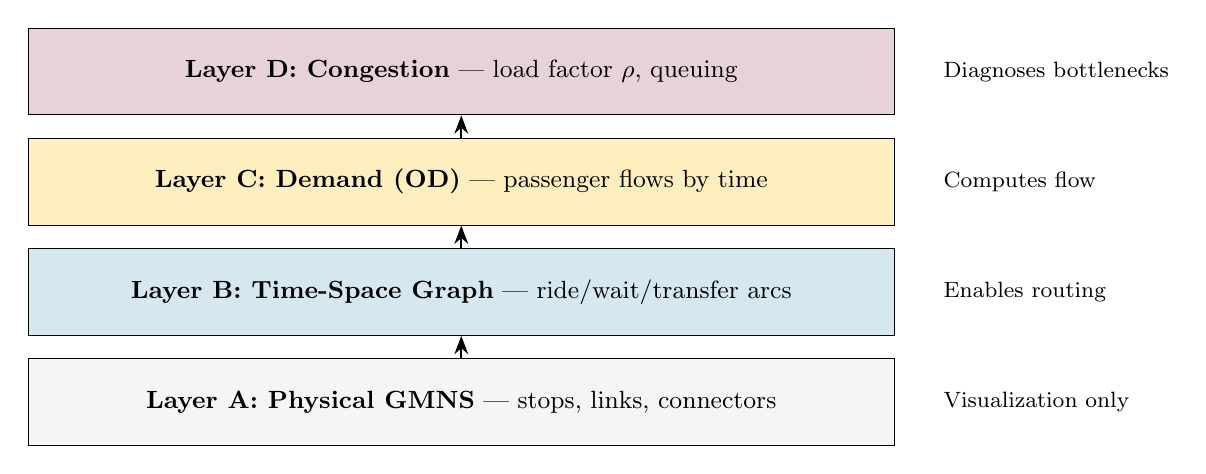
\begin{tikzpicture}[
    layer/.style={rectangle, draw, minimum width=11cm, minimum height=1.1cm, align=center, font=\small},
    arrow/.style={-Stealth, thick}
]
\node[layer, fill=lightgray] (A) at (0,0) {\textbf{Layer A: Physical GMNS} --- stops, links, connectors};
\node[layer, fill=lightblue] (B) at (0,1.4) {\textbf{Layer B: Time-Space Graph} --- ride/wait/transfer arcs};
\node[layer, fill=asugold!30] (C) at (0,2.8) {\textbf{Layer C: Demand (OD)} --- passenger flows by time};
\node[layer, fill=asumaroon!20] (D) at (0,4.2) {\textbf{Layer D: Congestion} --- load factor $\rho$, queuing};

\draw[arrow] (A) -- (B);
\draw[arrow] (B) -- (C);
\draw[arrow] (C) -- (D);

\node[right, font=\footnotesize] at (6,0) {Visualization only};
\node[right, font=\footnotesize] at (6,1.4) {Enables routing};
\node[right, font=\footnotesize] at (6,2.8) {Computes flow};
\node[right, font=\footnotesize] at (6,4.2) {Diagnoses bottlenecks};
\end{tikzpicture}
\end{center}

\begin{warningbox}{Critical Understanding}
Without Layer B (Time-Space Graph), students cannot answer \emph{any} operational question. Without Layer D (Congestion), they cannot answer ``where is it crowded and why?'' Simply producing \texttt{node.csv} and \texttt{link.csv} is \textbf{not} transit system modeling.
\end{warningbox}

%=============================================
\section{Phase 1: Digital Anatomy (Measurable Data Mastery)}
%=============================================

Students must prove they understand \emph{how} GTFS files create the time-space representation. This phase establishes the ``why'' behind every data element.

\begin{readingbox}{Required Reading for Phase 1}
\textbf{Primary:} Lecture 2.4 --- GTFS2GMNS User Guide, Sections 1--4\\
\textbf{Reference:} GTFS Official Specification (gtfs.org)
\end{readingbox}

\subsection{Module 1.1: The Stop-Link-Route Chain}

\begin{deliverablebox}{Deliverable 1.1: Physical Network Generation}
\textbf{Input Files:} \texttt{stops.txt}, \texttt{shapes.txt}, \texttt{routes.txt}\\
\textbf{Task:} Use GTFS2GMNS to generate the physical network\\
\textbf{Output:} Clean GMNS CSVs (\texttt{node.csv}, \texttt{link.csv})\\[0.3cm]
\textbf{Verification Checklist:}
\begin{itemize}[nosep]
    \item[$\square$] Number of physical nodes matches unique stops in \texttt{stops.txt}
    \item[$\square$] All routes are represented in service links
    \item[$\square$] Node coordinates are valid (lat/lon within expected range)
    \item[$\square$] Link geometries are properly formatted (WKT LineString)
\end{itemize}
\end{deliverablebox}

\begin{metricbox}{Metric 1.1: Circuitry Index}
The \textbf{Circuitry Index} measures route directness:
\[
\text{Circuitry} = \frac{\text{Route Length (along shape)}}{\text{Euclidean Distance (origin to terminus)}}
\]

\textbf{Calculation Steps:}
\begin{enumerate}[nosep]
    \item Extract route shape from \texttt{shapes.txt}
    \item Calculate total route length using Haversine formula between consecutive points
    \item Calculate straight-line distance between first and last stop
    \item Compute ratio
\end{enumerate}

\textbf{Interpretation:}
\begin{center}
\begin{tabular}{cl}
\toprule
\textbf{Value} & \textbf{Interpretation} \\
\midrule
$\approx 1.0$ & Direct express service \\
$1.2$--$1.5$ & Typical urban route \\
$> 2.0$ & Highly circuitous (coverage-oriented) \\
\bottomrule
\end{tabular}
\end{center}

\textbf{Question to Answer:} Why does the bus deviate? Is it for coverage (serving more people) or is there a constraint (road network, terrain)?
\end{metricbox}

\subsection{Module 1.2: Timetable to Service-Node Expansion}

This module connects to the \textbf{two-layer network structure} described in Lecture 2.4 (Section 4.1): the Service Layer and the Topological Layer.

\begin{deliverablebox}{Deliverable 1.2: Time-Space Diagram}
\textbf{Input File:} \texttt{stop\_times.txt}\\
\textbf{Task:} For \textbf{one selected stop}, enumerate all ``service nodes'' $(stop, time)$ between 7:00--9:00 AM\\
\textbf{Output:} 
\begin{itemize}[nosep]
    \item Time-space diagram (hand-drawn or generated)
    \item Table listing: trip\_id, arrival\_time, departure\_time, route\_id
    \item Headway calculation between consecutive arrivals
\end{itemize}
\end{deliverablebox}

\begin{metricbox}{Metric 1.2: Headway Deviation (Coefficient of Variation)}
Let $h_i$ be the headway (time gap) before arrival $i$, and $\bar{h}$ the mean headway:
\[
\text{CV}_h = \frac{\sigma_h}{\bar{h}} = \frac{\sqrt{\frac{1}{n}\sum_{i=1}^{n}(h_i - \bar{h})^2}}{\bar{h}}
\]

\textbf{Interpretation:}
\begin{center}
\begin{tabular}{cl}
\toprule
\textbf{CV Value} & \textbf{Service Quality} \\
\midrule
$< 0.2$ & Well-regulated service \\
$0.2$--$0.5$ & Moderate bunching \\
$> 0.5$ & Severe bunching (operational problem) \\
\bottomrule
\end{tabular}
\end{center}

\textbf{Connection to Practice:} In Lecture 2.1, Joe Gregory discusses how On-Time Performance suffers when drivers don't have enough run time or layover time. Your headway deviation metric quantifies this problem.
\end{metricbox}

%=============================================
\section{Phase 2: Operations \& Optimization}
%=============================================

This phase bridges data understanding to service planning decisions, directly applying concepts from Joe Gregory's Valley Metro presentation.

\begin{readingbox}{Required Reading for Phase 2}
\textbf{Primary:} Lecture 2.1 --- Valley Metro Service Planning (Joe Gregory)\\
\textbf{Focus Areas:}
\begin{itemize}[nosep]
    \item Slides 13--16: Scheduling/Blocking and Fiesta BUZZ Case Study
    \item Slides 17--21: Connecting to New Service (AV Pilot)
\end{itemize}
\textbf{Secondary:} Lecture 2.2 --- Bus and Driver Scheduling
\end{readingbox}

\subsection{Module 2.1: Interlining \& Vehicle Blocking}

\begin{conceptbox}{Concept: The Fiesta BUZZ Case Study (from Lecture 2.1)}
From Lecture 2.1 (Slide 14):
\begin{itemize}[nosep]
    \item New route introduced in October 2022
    \item 52 minutes of runtime round trip
    \item 2 vehicles being used
    \item \textbf{Problem:} On-Time Performance suffers from insufficient run time or layover time
\end{itemize}

\textbf{Solution (Slide 16):}
\begin{itemize}[nosep]
    \item Interline routes (DBUZ and FBUZ)
    \item Add one vehicle
    \item Adjust dwell time locations
\end{itemize}

This case study demonstrates that \texttt{stops.txt} locations and \texttt{stop\_times.txt} schedules are \textbf{decision variables}, not fixed constraints.
\end{conceptbox}

\begin{deliverablebox}{Deliverable 2.1: Deadhead Analysis}
\textbf{Task:} Identify blocking opportunities in your GMNS network\\[0.2cm]
\textbf{Specific Requirements:}
\begin{enumerate}[nosep]
    \item Find Trip A ending at time $t_1$ at stop $s_1$
    \item Find Trip B starting at time $t_2 > t_1$ at stop $s_2$ nearby
    \item Calculate:
    \begin{itemize}[nosep]
        \item Deadhead distance: $d(s_1, s_2)$ in meters
        \item Layover time: $t_2 - t_1$ in minutes
        \item Is layover $\geq$ minimum required (typically 5--10 min)?
    \end{itemize}
\end{enumerate}

\textbf{Optimization Question:} If you relocate stop $s_2$ by 200m in \texttt{stops.txt}, does deadhead decrease? Can this save a vehicle?
\end{deliverablebox}

\subsection{Module 2.2: Frequency vs. Fleet Size Trade-off}

\begin{conceptbox}{The Fundamental Fleet Equation}
From Lecture 2.2, the relationship between service frequency and fleet size:
\[
\boxed{N_{\text{buses}} = \frac{T_{\text{cycle}}}{h}}
\]
where:
\begin{align*}
T_{\text{cycle}} &= T_{\text{running}} + T_{\text{layover}} \quad \text{(round-trip cycle time)}\\
h &= \text{headway (time between buses)}\\
N_{\text{buses}} &= \text{number of vehicles required}
\end{align*}

\textbf{Implication:} Doubling frequency ($h \to h/2$) doubles fleet requirement ($N \to 2N$).
\end{conceptbox}

\begin{deliverablebox}{Deliverable 2.2: Fleet Optimization Under Constraint}
\textbf{Given:}
\begin{itemize}[nosep]
    \item A fixed fleet of $N = 10$ buses
    \item Current route with $T_{\text{running}} = 45$ min (one direction)
    \item Required layover: $T_{\text{layover}} = 8$ min at each terminal
\end{itemize}

\textbf{Tasks:}
\begin{enumerate}
    \item Calculate cycle time: $T_{\text{cycle}} = 2 \times 45 + 2 \times 8 = 106$ min
    \item Determine minimum achievable headway: $h_{\min} = T_{\text{cycle}} / N = 10.6$ min
    \item If you want 10-minute headway, how many buses do you need?
    \item \textbf{Optimization:} Propose a schedule modification in \texttt{stop\_times.txt} that achieves the highest frequency possible without exceeding 10 buses
\end{enumerate}

\textbf{Constraint:} Your solution must maintain minimum layover times for driver breaks.
\end{deliverablebox}

%=============================================
\section{Phase 3: Demand, Load, and Congestion}
%=============================================

This is where students prove the network is ``real'' by adding passengers. This phase directly implements the applications described in Lecture 2.4, Section 6.

\begin{readingbox}{Required Reading for Phase 3}
\textbf{Primary:} Lecture 2.4 --- GTFS2GMNS User Guide, Section 6 (Applications)\\
\textbf{Focus Areas:}
\begin{itemize}[nosep]
    \item Section 6.1: Traffic Assignment
    \item Section 6.5: Linear Programming Applications
\end{itemize}
\textbf{Reference:} Lecture 2.1, Slides 8--12: Origin and Destination Study
\end{readingbox}

\subsection{Module 3.1: Building the OD Layer}

From Lecture 2.1 (Joe Gregory), Valley Metro conducts O-D surveys every 3--5 years, collecting 17,000 completed surveys covering trip origin/destination, transfers, trip purpose, fare type, and access/egress modes.

\begin{deliverablebox}{Deliverable 3.1: Synthetic OD Matrix}
\textbf{Task:} Create a simple CSV representing 1,000 passenger trips\\[0.2cm]
\textbf{Required Fields:}
\begin{center}
\begin{tabular}{lll}
\toprule
\textbf{Field} & \textbf{Type} & \textbf{Description} \\
\midrule
trip\_id & integer & Unique passenger trip identifier \\
origin\_stop & string & Boarding stop (from \texttt{stops.txt}) \\
dest\_stop & string & Alighting stop \\
dep\_time & HH:MM & Desired departure time \\
\bottomrule
\end{tabular}
\end{center}

\textbf{Generation Method (choose one):}
\begin{enumerate}[nosep]
    \item \textbf{Gravity Model:} $T_{ij} = k \cdot \frac{P_i \cdot A_j}{d_{ij}^2}$ where $P_i$ = population near stop $i$, $A_j$ = jobs near stop $j$
    \item \textbf{Uniform Random:} Random selection of O-D pairs with peak-hour concentration
    \item \textbf{Census-Based:} Use ACS commute data if available
\end{enumerate}
\end{deliverablebox}

\subsection{Module 3.2: Load Profile and Congestion Detection}

\begin{deliverablebox}{Deliverable 3.2: Load Profile Graph}
\textbf{Output:} A graph showing passenger load along a route\\[0.2cm]
\textbf{Axes:}
\begin{itemize}[nosep]
    \item X-axis: Distance along route (or stop sequence)
    \item Y-axis: Number of passengers on vehicle
\end{itemize}

\textbf{Calculation:}
For each link $(i, j)$ on a trip:
\[
\text{Load}_{ij} = \text{Load}_{i-1,i} + \text{Boardings}_i - \text{Alightings}_i
\]

\textbf{Constraint Check:}
\[
\rho_{ij} = \frac{\text{Load}_{ij}}{\text{Capacity}} \leq 1.0
\]

If $\rho > 1.0$ (overcrowding), student must propose solution.
\end{deliverablebox}

\begin{metricbox}{Metric 3.1: Load Factor ($\rho$)}
The load factor measures vehicle utilization:
\[
\rho = \frac{\text{Passengers on arc}}{\text{Vehicle capacity}}
\]

\textbf{Interpretation and Action:}
\begin{center}
\begin{tabular}{cll}
\toprule
\textbf{$\rho$ Value} & \textbf{Status} & \textbf{Required Action} \\
\midrule
$< 0.5$ & Underutilized & Consider reducing frequency \\
$0.5$--$0.85$ & Healthy & Optimal operating range \\
$0.85$--$1.0$ & Near capacity & Monitor closely \\
$> 1.0$ & Overcrowded & \textbf{Must solve:} increase frequency or capacity \\
\bottomrule
\end{tabular}
\end{center}
\end{metricbox}

%=============================================
\section{Phase 4: Measuring Network ``Goodness''}
%=============================================

To ensure students aren't just doing ``busy work,'' they must compute and report standardized performance metrics.

\begin{readingbox}{Required Reading for Phase 4}
\textbf{Primary:} Lecture 2.4 --- Sections 6.3 (Accessibility) and 6.4 (Equity Analysis)\\
\textbf{Reference:} Lecture 2.1 --- Slides 5--7: System Perspectives (Riders, Operators, Funders)
\end{readingbox}

\subsection{Three Essential Performance Statistics}

\begin{metricbox}{Statistic 1: Stop Accessibility}
\textbf{Definition:} Percentage of population within 400m walking distance of a transit stop.

\[
\text{Accessibility} = \frac{\sum_{i \in \text{Stops}} \text{Pop}(\text{Buffer}_{400m}(i))}{\text{Total Population}} \times 100\%
\]

\textbf{Calculation Method:}
\begin{enumerate}[nosep]
    \item Extract stop coordinates from \texttt{node.csv}
    \item Create 400m buffer around each stop
    \item Overlay with census population data
    \item Compute coverage percentage
\end{enumerate}

\textbf{Benchmark:} Good urban transit systems achieve $>80\%$ coverage.
\end{metricbox}

\begin{metricbox}{Statistic 2: Effective Speed}
\textbf{Definition:} Average speed including all delays (dwell time, traffic, etc.)

\[
\text{Effective Speed} = \frac{\text{Total Route Distance}}{\text{Total Travel Time (including dwell)}}
\]

\textbf{Threshold Rule:}
\begin{itemize}[nosep]
    \item If Effective Speed $< 10$ mph, student must propose \textbf{Stop Consolidation}
    \item Stop Consolidation = deleting rows in \texttt{stops.txt} to reduce dwell time
    \item Must justify which stops to remove (low ridership, close spacing)
\end{itemize}
\end{metricbox}

\begin{metricbox}{Statistic 3: Transfer Penalty}
\textbf{Definition:} Average waiting time at transfer nodes (where multiple routes intersect)

\[
\text{Transfer Penalty} = \frac{1}{|T|} \sum_{t \in T} \left( \text{Departure}_{\text{connecting}} - \text{Arrival}_{\text{arriving}} \right)
\]

where $T$ is the set of all transfer opportunities.

\textbf{Connection to GMNS:} Transfer links in \texttt{link.csv} (link\_type = ``transferring'') connect physical stations. The penalty is encoded in \texttt{VDF\_penalty1}.

\textbf{Benchmark:} Well-coordinated systems achieve transfer penalties $< 10$ minutes.
\end{metricbox}

%=============================================
\section{Deliverable Checklist and Grading Rubric}
%=============================================

\subsection{Summary Checklist (交件 Template)}

\begin{center}
\begin{tabular}{|c|l|l|c|}
\hline
\rowcolor{darkblue}\textcolor{white}{\textbf{Step}} & \textcolor{white}{\textbf{Deliverable}} & \textcolor{white}{\textbf{What It Proves}} & \textcolor{white}{\textbf{Points}} \\
\hline
1 & Clean GMNS CSVs & Data pipeline competency & 15 \\
\hline
2 & Time-Space Diagram & Time-expanded logic understanding & 15 \\
\hline
3 & Vehicle Requirement Calc & Schedule-Cost link & 20 \\
\hline
4 & Congestion Heatmap & Network-Demand link & 25 \\
\hline
5 & Optimization Memo & Problem-solving ability & 25 \\
\hline
\multicolumn{3}{|r|}{\textbf{Total}} & \textbf{100} \\
\hline
\end{tabular}
\end{center}

\subsection{Detailed Rubric}

\subsubsection*{Deliverable 1: Clean GMNS CSVs (15 points)}
\begin{itemize}[nosep]
    \item (5 pts) \texttt{node.csv} contains correct physical and service nodes
    \item (5 pts) \texttt{link.csv} contains all four link types
    \item (5 pts) Data passes validation (no missing fields, valid geometries)
\end{itemize}

\subsubsection*{Deliverable 2: Time-Space Diagram (15 points)}
\begin{itemize}[nosep]
    \item (5 pts) Correct identification of service nodes for selected stop
    \item (5 pts) Accurate headway calculations
    \item (5 pts) CV calculation and interpretation
\end{itemize}

\subsubsection*{Deliverable 3: Vehicle Requirement (20 points)}
\begin{itemize}[nosep]
    \item (5 pts) Correct cycle time calculation
    \item (5 pts) Correct fleet size calculation
    \item (5 pts) Deadhead analysis with specific trip pairs
    \item (5 pts) Optimization proposal with quantified savings
\end{itemize}

\subsubsection*{Deliverable 4: Congestion Heatmap (25 points)}
\begin{itemize}[nosep]
    \item (5 pts) Valid OD matrix with 1,000 trips
    \item (10 pts) Correct load profile calculation
    \item (5 pts) Identification of overcrowded segments
    \item (5 pts) Visualization quality
\end{itemize}

\subsubsection*{Deliverable 5: Optimization Memo (25 points)}
\begin{itemize}[nosep]
    \item (5 pts) Clear problem statement
    \item (10 pts) Quantified before/after comparison
    \item (5 pts) Feasibility analysis (constraints respected)
    \item (5 pts) Professional writing quality
\end{itemize}

%=============================================
\section{Connection to Advanced Topics}
%=============================================

\subsection{From Transit to Multi-Modal Systems}

The framework presented here extends naturally to other transportation systems. The state-action-transition structure applies universally:

\begin{center}
\begin{tabular}{lccc}
\toprule
\textbf{System} & \textbf{State $s_t$} & \textbf{Action $a_t$} & \textbf{Capacity Evolution} \\
\midrule
Transit & Platform queue, vehicle load & Dispatch, hold & Boarding constraints \\
Airport Ground & Gate occupancy, taxiway load & Pushback, ground hold & Runway capacity \\
Airspace & Sector occupancy & Metering, reroute & Sector capacity \\
Power Grid & Line loading, reserve & Generation dispatch & Thermal limits \\
\bottomrule
\end{tabular}
\end{center}

\subsection{Linear Programming Formulation}

From Lecture 2.4 (Section 6.5), the GMNS network directly maps to LP models:

\textbf{Transit Assignment Problem:}
\begin{align}
\min \quad & \sum_{a \in A} \int_0^{x_a} t_a(\omega) \, d\omega \\
\text{s.t.} \quad & \sum_{p \in P_{rs}} f_p = q_{rs} \quad \forall (r,s) \in OD \\
& x_a = \sum_{p \in P} \delta_{ap} f_p \quad \forall a \in A \\
& x_a \leq u_a \quad \forall a \in A \\
& f_p \geq 0 \quad \forall p \in P
\end{align}

where:
\begin{itemize}[nosep]
    \item $A$: Set of links from GMNS network
    \item $x_a$: Flow on link $a$
    \item $t_a$: Travel time (from \texttt{VDF\_fftt1})
    \item $u_a$: Capacity (from \texttt{capacity} field)
\end{itemize}

%=============================================
\section{Appendix: Quick Reference}
%=============================================

\subsection{GTFS File Summary}

\begin{center}
\begin{tabular}{lll}
\toprule
\textbf{File} & \textbf{Key Fields} & \textbf{GMNS Mapping} \\
\midrule
\texttt{stops.txt} & stop\_id, stop\_lat, stop\_lon & Physical nodes \\
\texttt{routes.txt} & route\_id, route\_type & directed\_route\_id \\
\texttt{trips.txt} & trip\_id, route\_id, direction\_id & Service links \\
\texttt{stop\_times.txt} & arrival\_time, departure\_time & VDF\_fftt1 \\
\texttt{shapes.txt} & shape\_pt\_lat/lon, shape\_pt\_sequence & Link geometry \\
\bottomrule
\end{tabular}
\end{center}

\subsection{GMNS Link Types}

\begin{center}
\begin{tabular}{llll}
\toprule
\textbf{Link Type} & \textbf{From Node} & \textbf{To Node} & \textbf{Purpose} \\
\midrule
Service & Service node & Service node & In-vehicle travel \\
Boarding & Physical & Service & Passenger boards \\
Deboarding & Service & Physical & Passenger alights \\
Transfer & Physical & Physical & Walk between stops \\
\bottomrule
\end{tabular}
\end{center}

\subsection{Key Formulas}

\begin{tcolorbox}[colback=lightgray, colframe=darkblue]
\textbf{Circuitry:} $\displaystyle \frac{\text{Route Length}}{\text{Euclidean Distance}}$

\vspace{0.3cm}
\textbf{Headway CV:} $\displaystyle \frac{\sigma_h}{\bar{h}}$

\vspace{0.3cm}
\textbf{Fleet Size:} $\displaystyle N = \frac{T_{\text{cycle}}}{h}$

\vspace{0.3cm}
\textbf{Load Factor:} $\displaystyle \rho = \frac{\text{Passengers}}{\text{Capacity}}$

\vspace{0.3cm}
\textbf{Effective Speed:} $\displaystyle \frac{\text{Distance}}{\text{Total Time}}$
\end{tcolorbox}

\subsection{Reading Assignment Mapping}

\begin{center}
\begin{tabular}{lll}
\toprule
\textbf{Phase} & \textbf{Primary Reading} & \textbf{Key Sections} \\
\midrule
Phase 1 & Lecture 2.4 (GTFS2GMNS Guide) & Sections 1--4 \\
Phase 2 & Lecture 2.1 (Valley Metro) & Slides 13--21 \\
Phase 2 & Lecture 2.2 (Bus Scheduling) & All \\
Phase 3 & Lecture 2.4 (GTFS2GMNS Guide) & Section 6 \\
Phase 3 & Lecture 2.1 (Valley Metro) & Slides 8--12 \\
Phase 4 & Lecture 2.4 (GTFS2GMNS Guide) & Sections 6.3--6.4 \\
\bottomrule
\end{tabular}
\end{center}

\end{document}
